\section{大数据时代的技术hive}
\par首先我们要知道hive到底是做什么的。下面这几段文字很好的描述了hive的特性:
\begin{enumerate}[(1)]
\item hive是基于Hadoop的一个数据仓库工具,可以将结构化的数据文件映射为一张数据库表,并提供完整的sql查询功能,可以将sql语句转换为MapReduce任务进行运行。其优点是学习成本低,可以通过类SQL语句快速实现简单的MapReduce统计,不必开发专门的MapReduce应用,十分适合数据仓库的统计分析。
\item Hive是建立在Hadoop上的数据仓库基础构架。它提供了一系列的工具,可以用来进行数据提取转化加载(ETL),这是一种可以存储、查询和分析存储在Hadoop中的大规模数据的机制。Hive定义了简单的类SQL查询语言,称为HQL,允许熟悉SQL的用户查询数据。同时,这个语言也允许熟悉MapReduce的开发者开发自定义的mapper和reducer函数来处理内建的mapper和reducer无法完成的复杂的分析工作。
\end{enumerate}
\par 使用hive的命令行接口,感觉很像操作关系数据库,但是hive和关系数据库还是有很大的不同,下面比较下hive与关系数据库的区别,具体如下:
\begin{enumerate}[(1)]
\item hive和关系数据库存储文件的系统不同,hive使用的是hadoop的HDFS(hadoop的分布式文件系统),关系数据库则是服务器本地的文件系统;
\item hive使用的计算模型是mapreduce,而关系数据库则是自己设计的计算模型,一般是基于连接(Join)操作,索引($B^+$树上的查询);
\item 关系数据库都是为实时查询的业务进行设计的,而hive则是为海量数据做数据挖掘设计的,实时性很差;实时性的区别导致hive的应用场景和关系数据库有很大的不同,因此,hive一般是用于统计分析的,商业推荐系统中,实时性的要求没那么高。
\item Hive很容易扩展自己的存储能力和计算能力,这个是继承hadoop的,而关系数据库在这个方面要比数据库差很多。
\end{enumerate}
\subsection{hive的技术架构}
\par 由图\ref{fig-hive-1}~可知,hdfs和mapreduce是hive架构的根基。Hive架构包括如下组件:CLI(command line interface)、JDBC/ODBC、Thrift Server、WEB GUI、metastore和Driver(Complier、Optimizer和Executor),这些组件可以分为两大类:服务端组件和客户端组件。
\begin{figure}[htbp]
\centering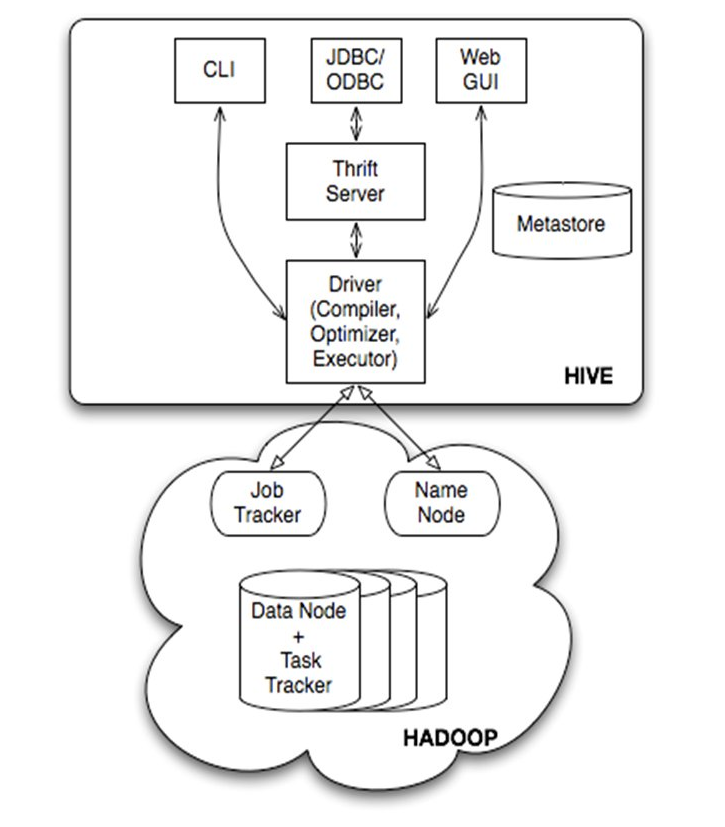
\includegraphics[width=.6\linewidth]{figures/hive.png}
\caption{hive基础架构图}\label{fig-hive-1}
\end{figure} 
\par \textbf{Driver}组件:该组件包括Complier、Optimizer和Executor,它的作用是将我们写的HiveQL(类SQL)语句进行解析、编译优化,生成执行计划,然后调用底层的mapreduce计算框架。
\par \textbf{Metastore}组件:元数据服务组件,这个组件存储hive的元数据,hive的元数据存储在关系数据库里,hive支持的关系数据库有derby、mysql。元数据对于hive十分重要,因此hive支持把metastore服务独立出来,安装到远程的服务器集群里,从而解耦hive服务和metastore服务,保证hive运行的健壮性。
\par \textbf{Thrift}服务:thrift是facebook开发的一个软件框架,它用来进行可扩展且跨语言的服务的开发,hive集成了该服务,能让不同的编程语言调用hive的接口。
客户端组件:

\par \textbf{CLI}:command line interface,命令行接口。
\par \textbf{Thrift客户端}:上面的架构图里没有写上Thrift客户端,但是hive架构的许多客户端接口是建立在thrift客户端之上,包括JDBC和ODBC接口。
\par \textbf{WEBGUI}:hive客户端提供了一种通过网页的方式访问hive所提供的服务。这个接口对应hive的hwi组件(hive web interface),使用前要启动hwi服务。
\par Hive的metastore组件是hive元数据集中存放地。Metastore组件包括两个部分:metastore服务和后台数据的存储。后台数据存储的介质就是关系数据库,例如hive默认的嵌入式磁盘数据库derby,还有mysql数据库。Metastore服务是建立在后台数据存储介质之上,并且可以和hive服务进行交互的服务组件,默认情况下,metastore服务和hive服务是安装在一起的,运行在同一个进程当中。也可以把metastore服务从hive服务里剥离出来,metastore独立安装在一个集群里,hive远程调用metastore服务,这样可以把元数据这一层放到防火墙之后,客户端访问hive服务,就可以连接到元数据这一层,从而提供了更好的管理性和安全保障。使用远程的metastore服务,可以让metastore服务和hive服务运行在不同的进程里,这样也保证了hive的稳定性,提升了hive服务的效率。
\begin{figure}[htbp]
\centering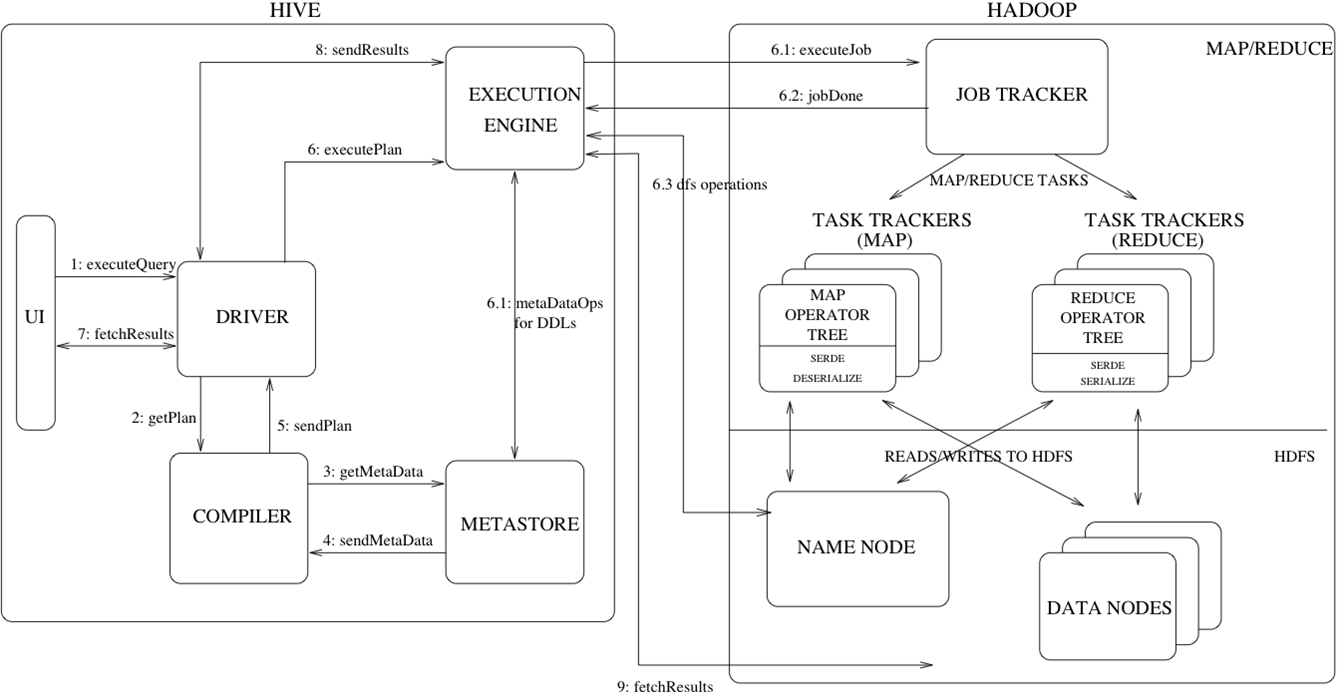
\includegraphics[width=\linewidth]{figures/hive-2.png}
\caption{hive执行流程}\label{fig-hive-2}
\end{figure} 
\subsection{hive与关系数据库的区别}
\par 关系数据库里,表的加载模式是在数据加载时候强制确定的(表的加载模式是指数据库存储数据的文件格式),如果加载数据时候发现加载的数据不符合模式,关系数据库则会拒绝加载数据,这个就叫“写时模式”,写时模式会在数据加载时候对数据模式进行检查校验的操作。Hive在加载数据时候和关系数据库不同,hive在加载数据时候不会对数据进行检查,也不会更改被加载的数据文件,而检查数据格式的操作是在查询操作时候执行,这种模式叫“读时模式”。在实际应用中,写时模式在加载数据时候会对列进行索引,对数据进行压缩,因此加载数据的速度很慢,但是当数据加载好了,我们去查询数据的时候,速度很快。但是当我们的数据是非结构化,存储模式也是未知时候,关系数据操作这种场景就麻烦多了,这时候hive就会发挥它的优势。
\par 关系数据库一个重要的特点是可以对某一行或某些行的数据进行更新、删除操作,hive不支持对某个具体行的操作,hive对数据的操作只支持覆盖原数据和追加数据。Hive也不支持事务和索引。更新、事务和索引都是关系数据库的特征,这些hive都不支持,也不打算支持,原因是hive的设计是海量数据进行处理,全数据的扫描是它的工作常态,针对某些具体数据进行操作的效率是很差的,对于数据的添加操作,hive是通过查询将原表的数据进行转化最后存储在新表里,这和传统数据库的更新操作有很大不同。
\par Hive也可以在hadoop做实时查询上做一份自己的贡献,那就是和hbase集成,hbase可以进行快速查询,但是hbase不支持类SQL的语句,那么此时hive可以给hbase提供sql语法解析的外壳,可以用类sql语句操作hbase数据库。今天的hive就写到这里,关于hive我打算一共写三篇文章,这是第一篇,下一篇主要讲hive支持的数据模型,例如:数据库(database)、表(table)、分区(partition)和桶(bucket),还有hive文件存储的格式,还有hive支持的数据类型。第三篇文章就会讲到hiveQL的使用、以及结合mapreduce查询优化的技术和自定义函数,以及我们现在在公司项目里运用hive的实例。马云在退休的时候说互联网现在进入了大数据时代,大数据是现在互联网的趋势,而hadoop就是大数据时代里的核心技术,但是hadoop和mapreduce操作专业型太强,所以facebook在这些的基础上开发了hive框架,毕竟世界上会sql的人比会java的人多的多,hive是可以说是学习hadoop相关技术的一个突破口,哪些自立于投身hadoop技术开发的童鞋们,可以先从hive开始哦。



